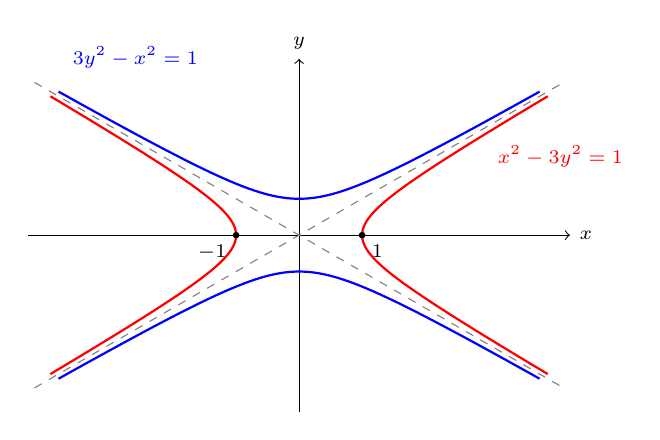
\begin{tikzpicture}[scale=0.8, every node/.style={font=\scriptsize}]
  \draw[->] (-4.3,0) -- (4.3,0) node[right] {$x$};
  \draw[->] (0,-2.8) -- (0,2.8) node[above] {$y$};
  \draw[gray, dashed] (-4.2,-2.425) -- (4.2,2.425);
  \draw[gray, dashed] (-4.2,2.425) -- (4.2,-2.425);
  \draw[red, thick, domain=-2.05:2.05, samples=60, variable=\u] plot ({cosh(\u)},{sinh(\u)/sqrt(3)});
  \draw[red, thick, domain=-2.05:2.05, samples=60, variable=\u] plot ({-cosh(\u)},{sinh(\u)/sqrt(3)});
  \draw[blue, thick, domain=-2.05:2.05, samples=60, variable=\u] plot ({sinh(\u)},{cosh(\u)/sqrt(3)});
  \draw[blue, thick, domain=-2.05:2.05, samples=60, variable=\u] plot ({sinh(\u)},{-cosh(\u)/sqrt(3)});
  \fill (1,0) circle (1.5pt) node[below right] {$1$};
  \fill (-1,0) circle (1.5pt) node[below left] {$-1$};
  \node[red, right] at (3.0,1.25) {$x^2-3y^2=1$};
  \node[blue, above] at (-2.6,2.5) {$3y^2-x^2=1$};
\end{tikzpicture}
